\section{Ergebnisse}
Abbildung \ref{filter} zeigt die für das Ausgangsfilter gemessenen Werte. Demnach beträgt die Dämpfung für die gewünschte Sendefrequenz 0,46dB. Die Dämpfung für die erste Oberschwingung beträgt etwa 45dB. Die in der Simulation berechneten Werte für das Filter waren 0dB für die Sendefrequenz und 46dB für die erste Oberschwingung. Die gemessenen Werte weichen also nur geringfügig davon ab und insgesamt erfüllt das Filter die Anforderungen.\\
\begin{figure}[H]\centering
	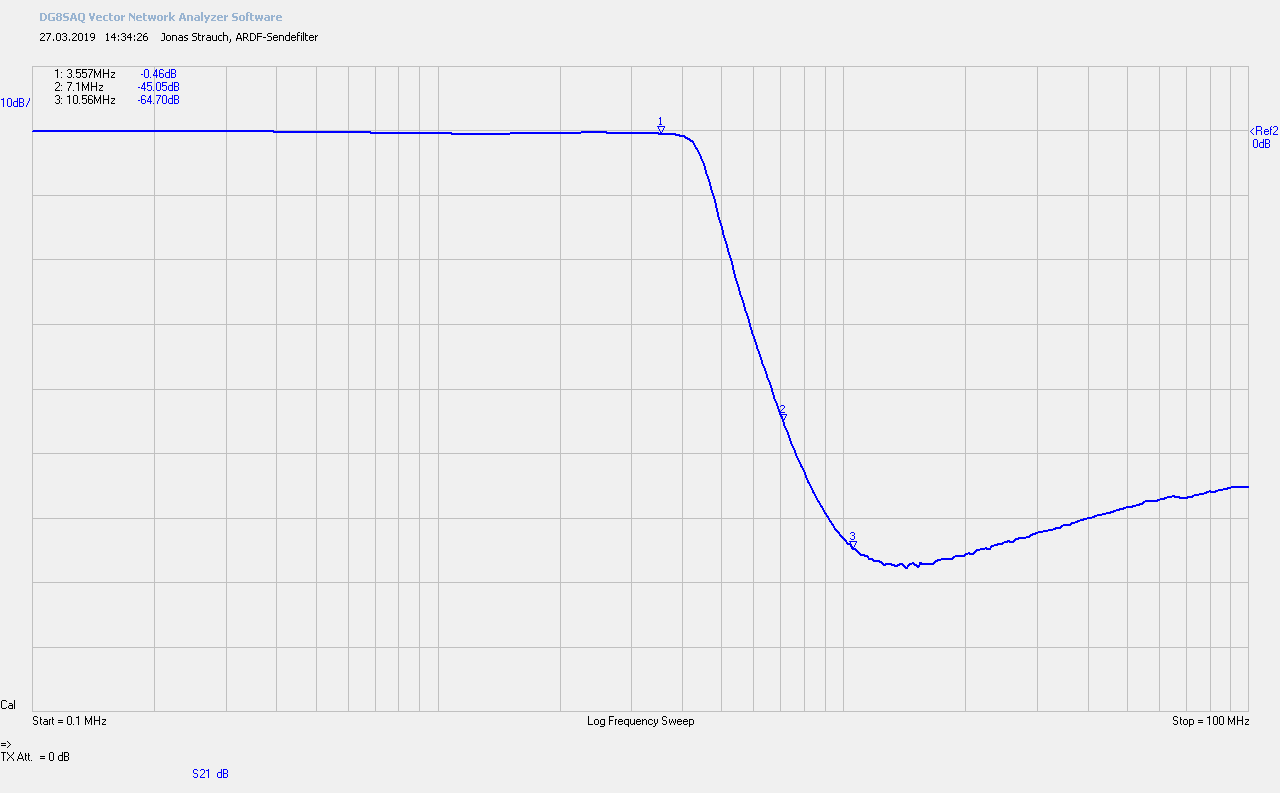
\includegraphics[width=16cm]{res/Filterwerte.png}
	\caption{Gemessene Werte des Ausgangsfilter}
	\label{filter}
\end{figure}

Die in der Validierung gemessene Sendeleistung beträgt 0,53W, was etwa der Hälfte des geforderten Werts entspricht. der Grund dafür scheint zu sein, dass der im Sender verwendete MOSFET nicht ganz auf Ground durchschaltet.
